% MODELO CONEM 2016
\documentclass[10pt,fleqn,a4paper]{article}
\usepackage{abcm}
\usepackage{float}

\begin{document}
    
    % CABEÇALHO
    \fancypagestyle{firststyle}
	{
   		\lhead{\emph{Anais do XXIV Encontro de Iniciação Científica e Pós-Graduação do ITA - XXV ENCITA / 2019\\
	Instituto Tecnológico de Aeronáutica, São José dos Campos, SP, Brasil, XXV 7 de novembro de 2019.}}  
	}
    \thispagestyle{firststyle}
    \vspace{-.5cm}
    \hspace{-.8cm}
    \begin{tabular}{p{\textwidth}}
    \begin{center}
    \vspace{-.6cm}
    \title{Otimização de parâmetros por meio de Algoritmos  Evolutivos  em Futebol de Robôs}
    \end{center}
    \textbf{Igor Mourão Ribeiro}\\
    \small{Instituto Tecnológico de Aeronáutica}\\
    \small{Rua H8A, 121, CTA}\\
    \small{12228-460 - São José dos Campos/SP}\\
    \small{Bolsista PIBIC - CNPq}\\
    \small{igormr98mr@gmail.com}\\
    \\ 
    \textbf{Celso Massaki Hirata}\\
    \small{Instituto Tecnológico de Aeronáutica}\\
    \small{Divisão de Ciência da Computação}\\
    \small{Praça Marechal Eduardo Gomes, 50}\\
    \small{12229-900 – São José dos Campos / SP}\\
    \small{hirata@ita.br}\\
    \\ 
    \textbf{Marcos Ricardo Omena de Albuquerque Máximo}\\
    \small{Instituto Tecnológico de Aeronáutica}\\
    \small{Divisão de Ciência da Computação}\\
    \small{Praça Marechal Eduardo Gomes, 50}\\
    \small{12.229-900 – São José dos Campos / SP}\\
    \small{maximo.marcos@gmail.com}\\
    \\
    \abstract{\textbf{Resumo:} O desenvolvimento de uma estratégia robusta e consistente para um time completo de robôs jogadores de futebol da categoria "Very Small Size" é fundamental para ganhar as partidas. Após uma fase de pesquisa, foi decidido usar o método da Behavior Tree (árvore de comportamentos) para realizar a tomada de decisões do time. Em seguida, foi escolhido três papeis para os jogadores: goleiro, principal e auxiliar. Depois, foi desenvolvido uma árvore de comportamentos para cada um deles, além de um técnico responsável por garantir troca dinâmica de papeis. O critério usado para avaliação do algoritmo foi o seu desempenho em partidas simuladas e em competições nacionais.}\\
    \keywords{\textbf{Palavras-chave:} robótica, estratégia, tomada de decisão}\\
    \end{tabular}

    \section{INTRODUÇÃO}
    No contexto do futebol de robôs, a otimização de parâmetros traz muitos desafios. Tal problema consiste no fato de se implementar um algoritmo que consiga encontrar as melhores constantes a serem usadas no código para melhorar o desempenho do robô em uma partida real. Entretando, para encontrar esses parâmetros de forma automatizada, é necessário, além do algoritmo evolutivo em si, a existência de simulações fiéis à realidade.

Nesse projeto, trabalhou-se com os robôs da competição IEEE Very Small Size (VSS): uma competição de futebol de robôs completamente automatizada em que cada robô tem como tamanho máximo um cubo de 7,5 cm de aresta. O campo de futebol possui 1,5 m de comprimento e 1,3 m de largura. Cada time tem 3 jogadores: que podem assumir posições dinâmicas, como goleiro e atacante, ao decorrer de uma partida. Uma câmera proporciona a visão aérea com as posições de todos os elementos da partida. As regras completas podem ser lidas em \cite{cbr2008}.

\begin{figure}[H]
	\centering
	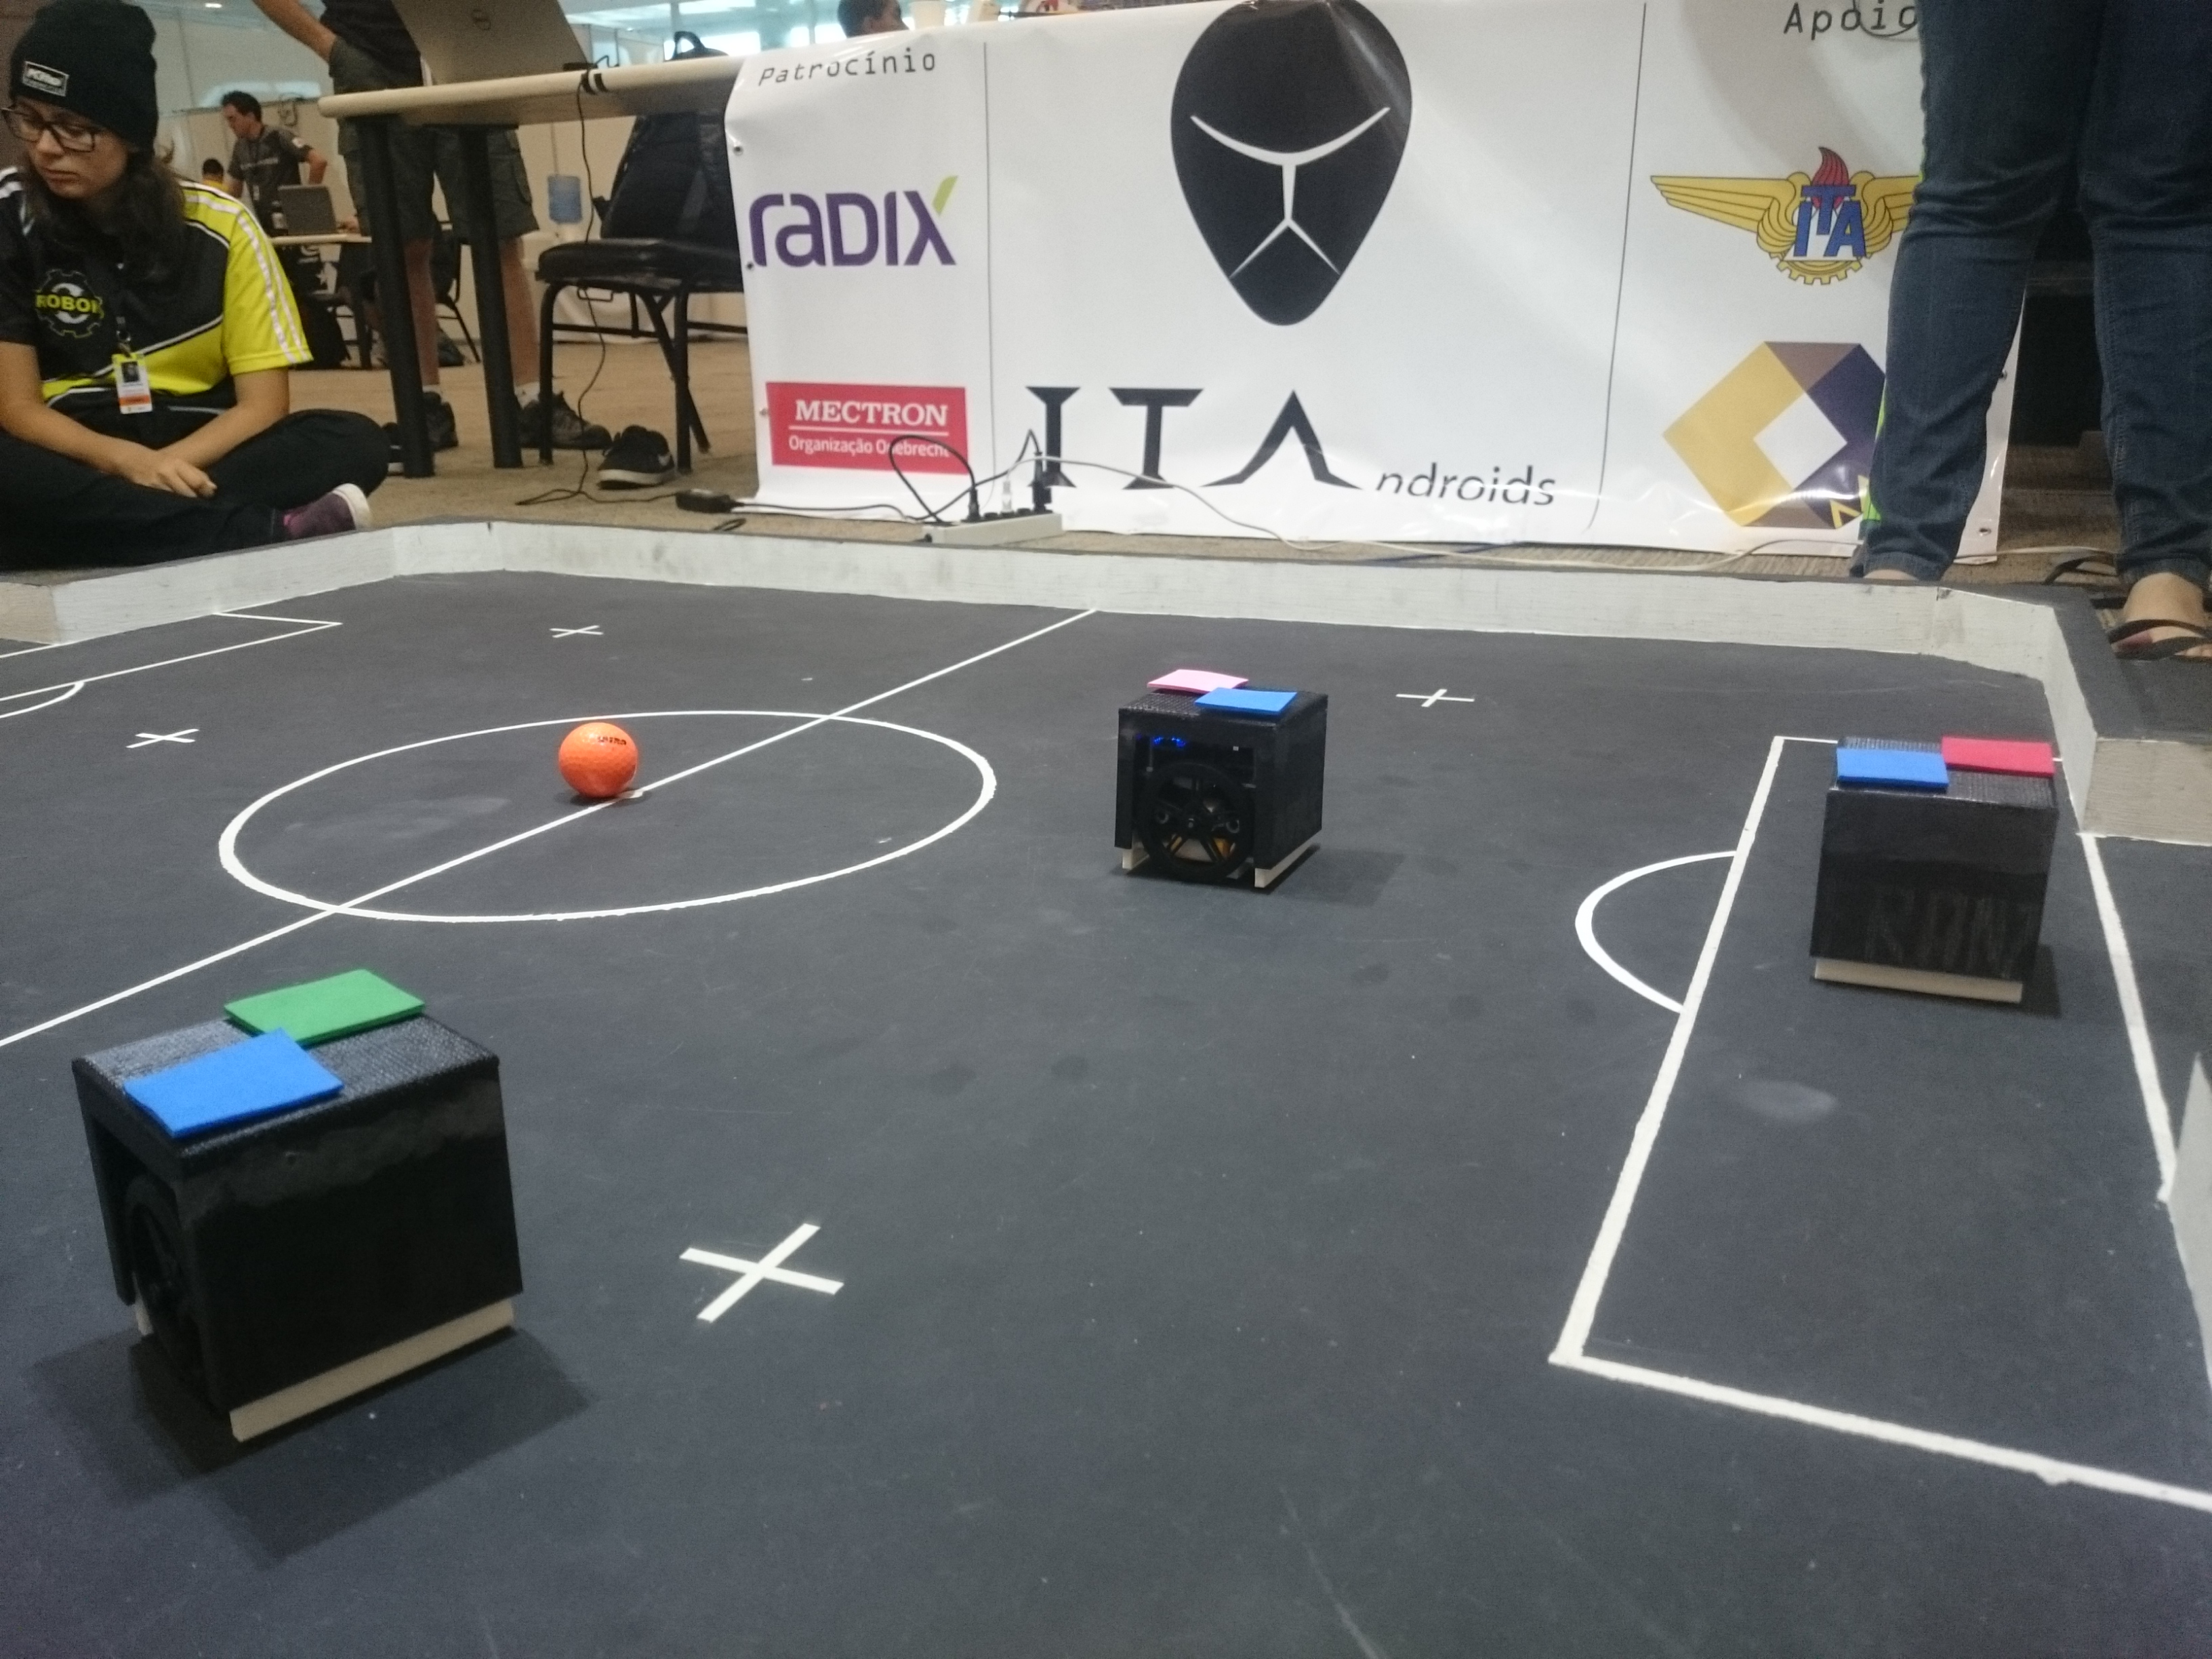
\includegraphics[width=0.5\textwidth]{figures/vss.JPG}
   \caption{Robôs da ITAndroids da categoria IEEE VSSS.} \label{fig:vss}
\end{figure}

A Figura \ref{fig:vss} mostra os robôs usados nas competições. A visão computacional utilizada pela equipe ITAndroids pode ser encontrada com mais detalhes em \cite{small_vision} e utiliza uma câmera no topo do campo que repassa informações para um computador processar, como visto na Figura \ref{fig:funcioamento}.

\begin{figure}[H]
	\centering
		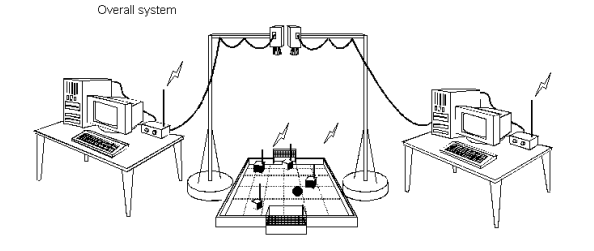
\includegraphics[width=0.7\textwidth]{figures/overview.png}
  \caption{Representação do funcionamento técnico de um jogo de VSS.}
	\label{fig:funcioamento}
\end{figure}

Cada robô foi projetado com duas rodas laterais e material teflon para diminuir atrito no deslizamento de seu chassis. Essa característica o torna um robô diferencial. Ou seja, temos o controle sobre as velocidades linear e angular, mas não é possível mover o robô para os lados. A linguagem utilizada para o projeto foi C++; diferente da utilizada nesse trabalho, que é Matlab; pois é uma linguagem que tem uma velocidade de execução alta e tem boa escalabilidade para um projeto grande. 

Nesse contexto, surgem várias questões a serem resolvidas para se ter um time vencedor. Nesse projeto, será abordado o seguinte problema de otimização: dado um simulador feito pela equipe que simula a física e a lógica de uma partida oficial, deve-se encontrar os melhores valores possíveis para as constantes do planejamento de trajetórias, de modo a maximizar o desempenho do time em uma partida com os robôs reais.

Sobre o assunto de planejamento de trajetórias, o utilizado pela equipe é o Univector Field \cite{univector}, que é muito eficiente e já demonstrou bons resultados em competições oficiais com algumas das melhores equipes utilizando-o. Uma das suas desvantagens, é a existência de sete parâmetros diferentes para serem otimizados e de que essas constantes não são intuitivas para uma pessoa ajustá-las sem ajuda de um computador. Isso acontece devido ao comportamento do algoritmo ser relativamente complexo quando comparado com outras alternativas como o algoritmo Campos Potenciais \cite{potential_fields}.

Além disso, é importante ressaltar que o tempo de execução do algoritmo deve ser o mínimo possível. Nota-se que não é possível simular uma partida completa de futebol já que isso demoraria bastante e o algoritmo precisa de em torno de 100 iterações para convergir. Para isso, técnicas para executar simulações aceleradas e executar situações específicas de jogo foram desenvolvidas, com o objetivo de reduzir o tempo total da otimização.

Ademais, outro problema que será enfrentado no desenvolvimento desse projeto é a criação de interfaces de comunicação entre o algoritmo de otimização, a ser codificado em Matlab, com o código do projeto e das simulações, ambos codificados na linguagem de programação C++.

Para resolver esse problema, foi escolhido como algoritmo para a otimização de parâmetros o Covariance Matrix Adaptation Evolution Strategy, já que ele consegue otimizar problemas não lineares e não convexos, que, devido à elevada complexidade, é o caso do futebol de robôs.

\subsection{Covariance Matrix Adaptation Evolution Strategy}

O algoritmo CMA-ES é uma estratégia evolutiva. Um algoritmo evolutivo é baseado no princípio da evolução biológica, em que conceitos de recombinação e mutação de genes são aplicados para selecionar melhores indivíduos. Mais formalmente: em cada geração novos indivíduos são criados a partir de seus pais, com o objetivo de gerar melhores indivíduos segundo algum critério.

No contexto da computação, cada geração será considerada uma iteração. Em cada iteração existirá uma população composta de indivíduos (ou candidatos) que deverá ser alterada segundo um algoritmo para diminuir uma determinada função de custo. 

Para o caso do CMA-ES, os novos indivíduos são escolhidos com base em uma distribuição gaussiana de múltiplas dimensões. A nova população será gerada a partir da média dos melhores indíviduos da população anterior, em combinação com uma perturbação gaussiana estocástica. Dependência entre diferentes parâmetros são representadas por uma matriz de covariâncias.

Nota-se que o algoritmo, brevemente descrito, não usa derivadas nem valores das funções de custo, apenas importa a comparação entre os desempenhos dos indíviduos de uma população.

\subsubsection{O algoritmo}

O algoritmo do CMA-ES pode ser separado em alguma etapas:

\begin{enumerate}
\item Escolha dos parâmetros iniciais para a otimização: o tamanho do passo, o ponto inicial, o tamanho da população e as condições de parada do algoritmo (que podem ser número de iterações ou ter um custo menor que um certo valor).
\item Enquanto a condição de parada não for atingida:
\begin{enumerate}
\item Gera novas soluções a partir da média dos melhores indivíduos da iteração anterior. Para isso usa-se uma distribuição gaussiana normal centrada em tal média e variância inicial igual ao tamanho do passo.
\item Cálculo dos custos de cada novo indivíduo por meio de uma função chamada de fitness.
\item Ordenação dos indíviduos, com base nos seus custos.
\item Atualização dos valores de variáveis internas.
\end{enumerate}
\end{enumerate}

Não será abordado os detalhes técnicos do item 2d, pois a implementação desse algoritmo não é o foco desse trabalho. Essa decisão ocorreu porque, além de tal passo ser bastante complexo estatisticamente, esse item apenas otimiza a velocidade de convergência do algoritmo e não é necessário para o entendimento inicial da estratégia evolutiva. Uma descrição mais profunda e detalhada de como otimizar o CMA-ES se encontra em \cite{CMA-ES}.

\subsection{O simulador}

Testes no robô real precisam de trabalho adicional devido a problemas que podem surgir como: bateria dos robôs acaba e precisa ser trocada, problemas no hardware ou mecânica do robô, campo sujo e necessidade de reposicionamento manual dos robôs. Por isso, a equipe ITAndroids desenvolveu um simulador próprio com o objetivo de resolver essas dificuldades.

O simulador é uma aplicação separada do código principal do time, desenvolvida e idealizada pela própria equipe, que cria um ambiente com física que simula um jogo. Tal aplicação se comunica com o código principal por meio de uma biblioteca de comunicação chamada Protocol Buffers \cite{protobuf}. Para isso, o simulador transmite informações como as posições e velocidades dos robôs para o código principal, enquanto que esse último transmite informações de velocidade das rodas de cada robô para o simulador.

A simulação foi desenvolvida em C++ com o auxílio da biblioteca Open Dynamics Engine \cite{ODE}, para fazer as computações das equações diferenciais da física e das colisões dos movimentos, e da biblioteca Ogre3D \cite{Ogre}, responsável por renderizar os objetos na tela em três dimensões. A Figura \ref{fig:simulator} mostra a interface visual do simulador logo antes de se começar uma partida.

\begin{figure}[H]
	\centering
	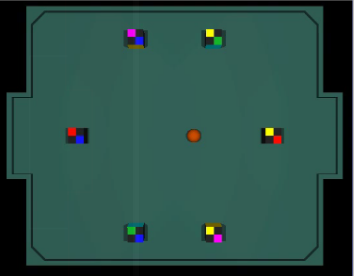
\includegraphics[width=0.6\textwidth]{figures/SimulatorWithoutButtons.png}
	\caption{Simulador da ITAndroids.}
	\label{fig:simulator}
\end{figure}


Com isso, é possivel ter uma aproximação do comportamento do time em um jogo real. Dado que o simulador é desenvolvido pela própria equipe, é possível adicionar situações especiais de jogo, além de se adicionar condições de paradas específicas para o que se deseja testar. Essas funcionalidades são muito importantes para a criação de situações específicas de jogo e, consequentemente, de funções de custo mais rápidas e otimizadas, o que garante uma convergência mais rápida de determinados parâmetros.

Além disso, o simulador também tem um modo de funcionar que é o chamado: modo acelerado. Normalmente, o código tem algumas funções para esperar um determinado tempo, com o objetivo de fazer que ele execute em tempo real (se ele não tivesse, a física seria muito rápida). Porém, no modo acelerado, esses tempos ociosos são removidos e a comunicação com o código principal funciona de forma assíncrona, o que garante uma velocidade de executação e simulação muito mais rápida, chegando a ser até dez vezes mais rápida que o modo de execução normal. Por essas razões, o modo acelerado é fundamental para garantir que a função de custo a ser desenvolvida seja mais eficiente e veloz.

\subsection{Univector Field}

O Univector Field é o planejamento de trajetórias usado pela equipe. O problema a ser resolvido é: como chegar de um ponto inicial à um ponto destino dentro do campo, desviando de obstáculos e considerando as limitações de controle e físicas do robô. Não será detalhado o funcionamento completo do algoritmo do Univector Field, já que isso pode ser visto em \cite{univector}.

Entretando, será descrito o que cada constante do algoritmo faz e uma descrição prática de como ela influencia na trajetória calculada, de modo a entender os resultados obtidos na otimização. Tem-se as seguinte constantes a serem otimizadas:
\begin{enumerate}
\item de: É o dobro de distância entre os centros de rotação do Univector Field. Na prática, quanto maior o seu valor, menos preciso o robô é em chegar em seu alvo. Se o seu valor for muito pequeno, o agente pode ficar preso em um mínimo local e nunca chegar em seu objetivo.
\item Kr: Define o quanto de rotação o campo gerado terá apontando para o seu alvo. Valores muito altos nessa constantes podem exigir que o robô faça curvas mais abruptas do que é possível e valores muito baixo farão que o robô faça curvas com raio muito grande, demorando mais a chegar no ponto desejado.
\item sigma: Parâmetro que define o tamanho do campo de repulsão gaussiano que o robô sofre de um obstáculo. Quanto maior o valor dessa constante, maior a repulsão do obstáculo.
\item dmin: A distância que o robô deve estar do obstáculo para o seu campo ser considerado infinito. Esse valor serve para garantir que o agente não colida com um obstáculo e deve ser otimizado para garantir que, se o robô se aproximar demais de um obstáculo, que ele seja repelido imediatamente e com muita intensidade.
\item K0: O parâmetro de predição de velocidade de obstáculos. É basicamente uma constante que é multiplicada pela velocidade do obstáculo para se calcular qual posição ele estará quando o agente chegar no objetivo. Único parâmetro que trata de obstáculos em movimento.
\item sigmaLine: Mesmo que o parâmetro sigma só que para as paredes do campo. As paredes são tratadas como um obstáculo especial já que, enquanto um obstáculo normal é um ponto, uma parede é uma reta.
\item dminLine:  O mesmo que a constante dmin só que para as paredes.
\end{enumerate}

O Univector Field é integrado com a interface de depuração da equipe, o que ajuda, qualitativamente, a verificar o quão otimizado é uma determinada trajetória gerada pelo algoritmo. Isso faz com que seja simples e rápido fazer uma checagem manual para saber se as constantes que o algoritmo convergiu não são absurdas.

\begin{figure}[H]
	\centering
	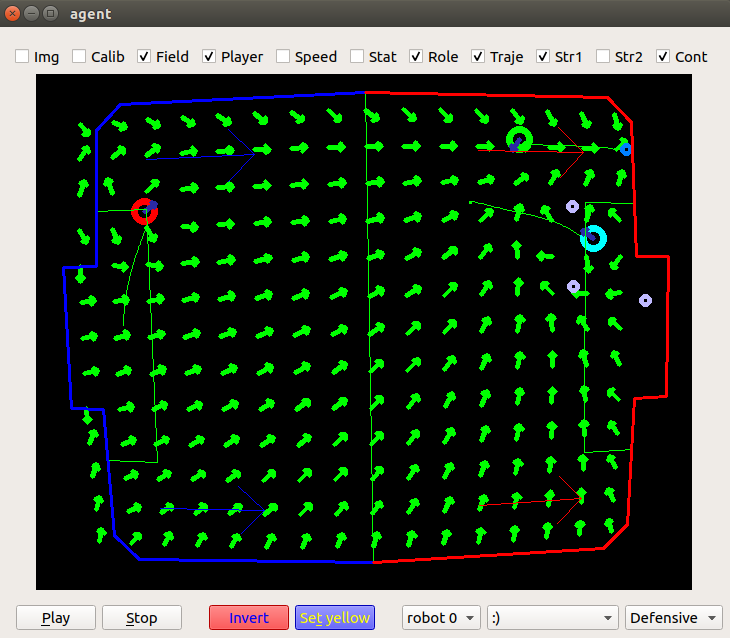
\includegraphics[width=0.83\textwidth]{figures/UnivectorFieldSimulatorDebugger.png}
	\caption{Interface gráfica para depuração da equipe}
	\label{fig:univector}
\end{figure}

Na Figura \ref{fig:univector}, é possível observar, em um determinado instante, as trajetórias calculadas para cada jogador e os vetores do campo do Univector Field para o jogador verde.


    \section{RESULTADOS OBTIDOS}
        
	Os resultados a seguir foram obtidos estudando o comportamentos de equipes adversárias na competição, além de diversos testes com o time de robôs da ITAndroids contra si mesmo em simulações computacionais em um simulador feito pela própria equipe, como mostrado na Figura \ref{fig:simulator}.

\begin{figure}[H]
	\centering
	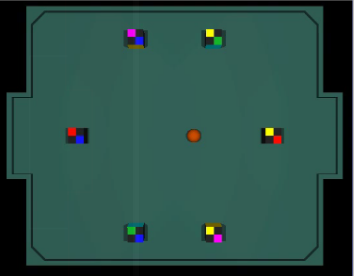
\includegraphics[width=0.6\textwidth]{figures/SimulatorWithoutButtons.png}
	\caption{Simulador da ITAndroids.}
	\label{fig:simulator}
\end{figure}

\subsection{Goleiro}

O goleiro é o jogador que deve ficar próximo ao gol aliado com o objetivo de proteger o gol de ataques oponentes. 
A BT criada para o goleiro está representada na Figura \ref{fig:goalier_bt}.

\begin{figure}[H]
	\centering
	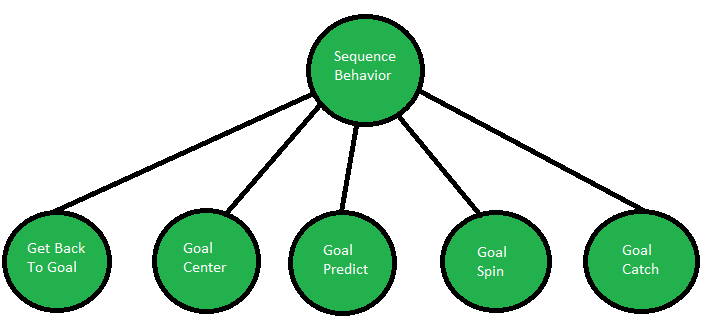
\includegraphics[width=0.8\textwidth]{figures/Goalier_BT.png}
   	\caption{Behavior Tree para o goleiro.} \label{fig:goalier_bt}
\end{figure}

Como visto, ela é composta por um nó do tipo Sequence Behavior, que irá executar os seus filhos em sequência. Esse papel, então, executa as seguintes ações prioritando as primeiras a aparecerem na seguinte lista:

\begin{itemize}

\item \textbf{Get Back to Goal Behavior} Volta para o gol, caso que, se por algum motivo ele esteja fora do próprio.

\item \textbf{Goal Center} Fica centralizado no gol quando a bola estiver longe, de forma que o jogador possa rapidamente ir para qualquer um dos lados quando a bola se aproximar.

\item \textbf{Goal Predict} Prediz para onde a bola irá quando ela estiver rápida e longe do gol.

\item \textbf{Goal Spin} Gira quando está perto da bola e não tem oponente perto da bola para jogá-la para longe.

\item \textbf{Goal Catch} Comportamento que o goleiro deverá fazer quando não fizer nenhum outro, por isso sua última posição na sequência. Ele acompanha o movimento da bola com o goleiro sobre a linha do gol.

\end{itemize}



\subsection{Principal}

O jogador com o papel de Principal é o jogador mais ativo do time, que deve estar constantemente avançando em direção a bola. Esse papel e o goleiro são as únicas posições que efetivamente deverão tocar na bola. A árvore \ref{fig:principal_bt} foi desenvolvida para o principal, sendo a árvore mais complexa dentre os papéis.

\begin{figure}[H]
	\centering
	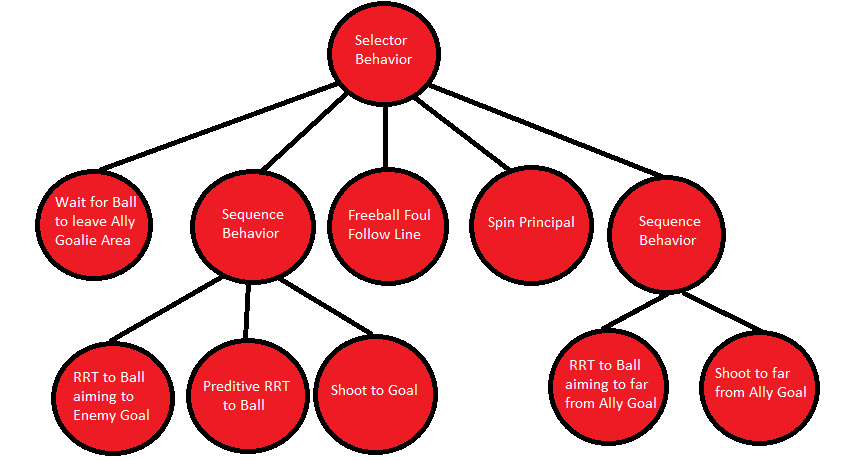
\includegraphics[width=0.8\textwidth]{figures/Principal_BT.png}
   	\caption{Behavior Tree para o principal.} \label{fig:principal_bt}
\end{figure}   

Conforme a Figura \ref{fig:principal_bt}, a raiz da árvore do principal é um Selector Behavior que escolhe uma das ações a ser realizada. Essa BT tem mais dois outros nós compostos, que são dois Sequence Behavior usados para o posicionamento atrás da bola, seguido pelo chute. Uma descrição dos nós folha utilizados se encontra abaixo:

\begin{itemize}

\item \textbf{Wait for Ball to leave Ally Goalie Area} Esse Behavior utiliza a Triangução de Delaunay. Esse comportamento deve evitar que o jogador entre na área do goleiro para não sofrer penâlti, conforme descrito na Figura \ref{fig:penalty}. O jogador se pocionará de acordo com posições escolhidas pelo usuário, calibradas com um arquivo de configuração .txt.

\begin{figure}[H]
	\centering
	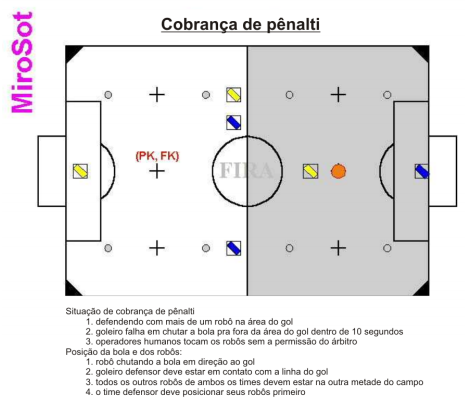
\includegraphics[width=0.7\textwidth]{figures/campo_penalty.png}
   \caption{Descrição da penalidade pênalti.} \label{fig:penalty}
\end{figure}

\item \textbf{RRT to Ball aiming to Enemy Goal} Irá usar o algoritmo de planejamento de trajetórias RRT para se deslocar atrás da bola com direção apontando para o gol oponente. Usado para se aproximar da bola e, em seguida, trocar para o próximo behavior, o Predictive RRT to Ball.

\item \textbf{Predictive RRT to Ball} Usa uma predição linear considerando que a bola continuará na mesma velocidade. Usado para se chegar na bola com mais precisão quando próximo a ela. Chega atrás da bola mirando para o gol.

\item \textbf{Shoot to Goal} Esse behavior só é chamado quando o jogador já está alinhado com a bola e o gol oponente. Esse comportamento acelera rapidamente o robô em linha reta para chegar no gol com uma velocidade alta.

\item \textbf{Free Ball Foul Follow Line} Esse behavior é um específico para situações de falta do tipo Bola Livre, conforme descrito na Figura \ref{fig:bola_livre}. Quando for detectado uma dessas posições, o jogador deve acelerar o mais rápido possível em direção à bola para ter o controle dela antes do oponente.

\begin{figure}[H]
	\centering
	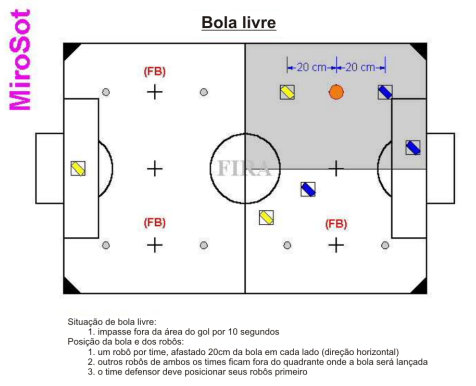
\includegraphics[width=0.7\textwidth]{figures/bola_livre.png}
   \caption{Descrição da penalidade bola livre.} \label{fig:bola_livre}
\end{figure}

\item \textbf{Spin Principal} Esse nó deve ser chamado quando a bola estiver em um dos quatros campos do campo. Caso seja um campo defensivo, o jogador irá girar para jogar a bola para frente; caso seja um na zona de ataque, o jogador girará para por a bola no centro do campo e continuar o ataque.

\item \textbf{RRT to Ball aiming to far from Ally Goal} Irá usar o algoritmo de planejamento de trajetórias RRT para se deslocar atrás da bola com direção apontando para a zona de ataque (longe do gol aliado). Usado para se aproximar da bola e se posicionar para, em seguida, chamar o Behavior Shoot to Far from Ally Goal.

\item \textbf{Shoot to Far from Ally Goal} Esse behavior só é chamado quando o jogador já está alinhado com a bola e o para frente (para longe do gol aliado). Esse comportamento acelera rapidamente o robô em linha reta para pôr a bola na zona de ataque.

\end{itemize}


\subsection{Auxiliar}

	O auxiliar é um papel que tem apenas uma função: posicionar-se da melhor forma possível para manter um ataque consistente. A ideia é que, caso a situação seja oportuna, o auxiliar se torne o principal e comece a atacar a bola. Para escolher a posição que o auxiliar deverá ficar em uma determinada situação de jogo, foi utilizado a Triangulação de \cite{delaunay34} sobre o grafo de \cite{voronoi08}. Esse algoritmo foi aplicado similarmente a \cite{akiyama2007multi}, relativo também à futebol de robôs.

	A Behavior Tree do auxiliar, por sua vez, é muito simples, representada por apenas um nó que tem como função se posicionar em lugar ótimo. Sua árvore, é representada simplesmente pela Figura \ref{fig:auxiliar_bt}.

\begin{figure}[H]
	\centering
	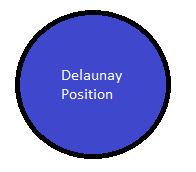
\includegraphics[width=0.3\textwidth]{figures/Auxiliar_BT.png}
   \caption{Behavior Tree para o auxiliar.} \label{fig:auxiliar_bt}
\end{figure}

	\section{CONCLUSÕES}
	Nesse artigo, apresentou-se uma implementação do método Behavior Tree para a categoria de futebol de robôs Very Small Size Soccer, que foi descrita, brevemente, o seu funcionamento. Foi mostrado o esquema de papéis utilizado bem como a Árvore de Comportamentos implementada para cada um deles, além de uma descrição detalhada sobre todos os nós das árvores.
	
	O projeto de Iniciação Científica apresentou bons resultados, especialmente quanto à vitória da equipe do ITA até às quartas de final da CBR 2017, rendendo o sétimo lugar à equipe dentre mais de 25 equipes participantes. Além do fato de que a ITAndroids conquistou o primeiro lugar na competição nacional de VSSS Copa Turing 2017, que ocorreu no final de setembro de 2017.

	Do ponto de vista técnico, o uso do algoritmo da Behavior Tree, já consagrado e usado por times de nível mundial, se mostrou factível e funcional em partidas reais de competições. Contudo, problemas como pouca escalabilidade e pouca reutilizabilidade se mostraram presentes na estratégia desenvolvida. Isso significa que mudanças ainda deverão ser feitas nas BT, principalmente a respeito do uso de mais nós do tipo paralelo para remover esses problemas citados.

    \section{AGRADECIMENTOS}
    
	Agradeço ao CNPq, pelo apoio financeiro e motivacional.
	
	Agradeço à ITAndroids, equipe que representa o ITA na competição da LARC/CBR, pela ideia do projeto, pela disponibilidade do robô real para implementação e oportunidade de aplicação dos métodos estudados.

	Agradeço ao professor doutor Paulo Marcelo Tasinaffo, meu orientador, e ao professor doutor Marcos Ricardo de Omena Máximo, co-orientador, ambos da Divisão da Ciência da Computação do ITA, pelo apoio nos estudos e no desenvolvimento do projeto.

    % REFERÊNCIAS
    \section{REFERÊNCIAS}
        \bibliographystyle{abcm}
        \bibliography{bibliografia}

    \section{RESPONSABILIDADE AUTORAIS}
    
        Os autores são os únicos responsáveis pelo conteúdo deste trabalho.

\end{document}